\documentclass{amsart}
%DIF LATEXDIFF DIFFERENCE FILE
%DIF DEL report_old.tex   Mon Apr 26 10:22:57 2021
%DIF ADD report.tex       Mon Apr 26 10:22:57 2021
\synctex=1

%=================================================================
% 
\newcount\DraftStatus  % 0 suppresses notes to selves in text
\DraftStatus=1   % TODO: set to 0 for final version
%=================================================================

%=================================================================
\usepackage{comment}
%=================================================================
%
\includecomment{JournalOnly}  
\includecomment{ConferenceOnly}  
\includecomment{TulipStyle}
%
%=================================================================
%=================================================================
% gitlatexdiff
%
%  https://gitlab.com/git-latexdiff/git-latexdiff
%=================================================================
%  git latexdiff HEAD  HEAD~5 --main templatex.tex
%  git latexdiff HEAD~1  --main templatex.tex
%  View pdf to see difference
%
%=================================================================
%
% Todo Notes for marginal comments
% 
%\newcount\DraftStatus  % 0 suppresses notes to selves in text
%\DraftStatus=1   % TODO: set to 0 for final version
\ifnum\DraftStatus=1
	\usepackage[draft,colorinlistoftodos,color=orange!30]{todonotes}
\else
	\usepackage[disable,colorinlistoftodos,color=blue!30]{todonotes}
\fi 
%\usepackage[disable]{todonotes} % notes not showed
%\usepackage[draft]{todonotes}   % notes showed
%
\makeatletter
 \providecommand\@dotsep{5}
 \def\listtodoname{List of Todos}
 \def\listoftodos{\@starttoc{tdo}\listtodoname}
 \makeatother
%
%=================================================================
%
\usepackage{color}
\newcommand{\draftnote}[3]{ 
	\todo[author=#2,color=#1!30,size=\footnotesize]{\textsf{#3}}	}
% TODO: add yourself here:
%
\newcommand{\gangli}[1]{\draftnote{blue}{GLi:}{#1}}
\newcommand{\PengChengJiang}[1]{\draftnote{red}{QWu:}{#1}}

\newcommand{\gliMarker}
	{\todo[author=GLi,size=\tiny,inline,color=blue!40]
	{Gang Li has worked up to here.}}
\newcommand{\pcjiangMarker}
	{\todo[author=PengCheng Jiang,size=\tiny,inline,color=red!40]
	{PengCheng Jiang has worked up to here.}}
%=================================================================

%=================================================================
%
% general packages
%  https://en.wikibooks.org/wiki/Category:Book:LaTeX
%  https://en.wikibooks.org/wiki/LaTeX/Package_Reference
%
%=================================================================
\usepackage{graphicx}
\usepackage{algorithm}
\usepackage{algorithmic}
\usepackage{breqn}
\usepackage{subcaption}
\usepackage{multirow}
\usepackage{psfrag}
\usepackage{url}
\usepackage{hyperref}
%\usepackage[colorlinks]{hyperref}
%\usepackage{cite}
\usepackage{cleveref}
\usepackage{booktabs}
\usepackage{rotating}
\usepackage{colortbl}
\usepackage{paralist}
%\usepackage{geometry}
\usepackage{epstopdf}
\usepackage{nag}
\usepackage{microtype}
\usepackage{siunitx}
\usepackage{nicefrac}
\usepackage{breakurl}
\usepackage{fontawesome}
\usepackage{xcolor}
\usepackage{multicol}
\usepackage{wrapfig}
\usepackage{todonotes}
\usepackage{tablefootnote}
\usepackage{threeparttable}
% for random text
\usepackage{lipsum}
\usepackage[english]{babel}
\usepackage[pangram]{blindtext}
% for tikz figures
\usepackage{tikz}
\usetikzlibrary{fit,positioning,arrows.meta,shapes,arrows}
%\tikzset{neuron/.style={circle,thick,fill=black!25,minimum size=17pt,inner sep=0pt},
%	input neuron/.style={neuron, draw,thick, fill=gray!30},
%	hidden neuron/.style={neuron,fill=white,draw},
%	hoz/.style={rotate=-90}}
%
%=================================================================



\begin{TulipStyle}
\usepackage[numbers]{natbib}
%=================================================================
%
% Version control information
%
%=================================================================
\usepackage{gitinfo2}
%=================================================================
\usepackage{fancyhdr}
\pagestyle{fancy}
\fancyhead{} % clear all header fields
\fancyhead[RO,LE]{\textsl{\rightmark}}
\fancyhead[LO,RE]{\ensuremath{\Rightarrow}
		\textbf{\textbf{[CONFIDENTIAL]}}\ensuremath{\Leftarrow}}
\fancyhead[CO,CE]{}
%=================================================================
\fancyfoot{} % clear all footer fields
\fancyfoot[CE,CO]{\textbf{\thepage}} 
\fancyfoot[LO,LE]{
\includegraphics[height=.9\headheight]{logos/tulip-logo.eps}
		\gitVtagn-\gitBranch\ (\gitCommitterDate)}
\fancyfoot[RO,RE]{Committed by: \textsl{\gitCommitterName}}

\setlength{\headheight}{12pt}
\renewcommand{\headrulewidth}{0.4pt}
\renewcommand{\footrulewidth}{0.4pt}
%=================================================================


%=================================================================
% for math notations
% ----------------------------------------------------------------
\usepackage{mathtools}
\usepackage{amsthm}
%
% THEOREMS -------------------------------------------------------
%
\newtheorem{thm}{Theorem}[section]
\newtheorem{cor}[thm]{Corollary}
\newtheorem{lem}[thm]{Lemma}
\newtheorem{prop}[thm]{Proposition}
\theoremstyle{definition}
\newtheorem{defn}[thm]{Definition}
\theoremstyle{remark}
\newtheorem{rem}[thm]{Remark}
\numberwithin{equation}{section}
% MATH -----------------------------------------------------------
\newcommand{\norm}[1]{\left\Vert#1\right\Vert}
\newcommand{\abs}[1]{\left\vert#1\right\vert}
\newcommand{\set}[1]{\left\{#1\right\}}
\newcommand{\Real}{\mathbb R}
\newcommand{\eps}{\varepsilon}
\newcommand{\To}{\longrightarrow}
\newcommand{\BX}{\mathbf{B}(X)}
% ----------------------------------------------------------------
\newcommand{\I}{{\cal I}}
\newcommand{\Id}{{\cal I} }
\newcommand{\Dc}{{\cal D}}
\newcommand{\J}{{\cal J}}
\newcommand{\Dn}{{\cal D}_n}
\newcommand{\Dd}{{\cal D}_n }
\renewcommand{\P}{{\cal P}}
\newcommand{\Nu}{{\cal N} }
\newcommand{\B}{{\cal B}}
\newcommand{\Bf}{{\bf B}}
\newcommand{\Y}{{\bf Y}}
\newcommand{\A}{{\cal A}}
% ----------------------------------------------------------------
\newcommand{\V}{{\cal V}}
\newcommand{\M}{{\cal M}}
\newcommand{\F}{{\cal F}}
\newcommand{\Fd}{{\cal F}}
\newcommand{\BF}{{\cal BF}_n}
\newcommand{\BFd}{{\cal BF}_n}
\newcommand{\TF}{{\cal TF}_n}
\newcommand{\TFd}{{\cal TF}_n}
%\newcommand{\G}{{\cal G}}
\newcommand{\X}{{\cal X}}
\newcommand{\E}{{\cal E}}
\newcommand{\K}{{\cal K}}
\newcommand{\T}{{\cal T}_n}
\renewcommand{\H}{{\cal H}}
% ----------------------------------------------------------------
\newtheorem{Remark}{Remark}
\newtheorem{proposition}{Proposition}
\newtheorem{theorem}{Theorem}
\newtheorem{lemma}{Lemma}
\newtheorem{corollary}{Corollary}
\newtheorem{example}{Example}
\newtheorem{definition}{Definition}
\newtheorem{Algorithms}{Algorithm}
% ----------------------------------------------------------------
\newcommand{\bu}{{\mathbf 1} }
\newcommand{\bo}{{\mathbf 0} }
\newcommand{\N}{\mbox{{\sl l}}\!\mbox{{\sl N}}}
% ----------------------------------------------------------------
\def\uint{[0,1]}
\def\proof{{\scshape Proof}. \ignorespaces}
\def\endproof{{\hfill \vbox{\hrule\hbox{%
   \vrule height1.3ex\hskip1.0ex\vrule}\hrule
  }}\par}
%
%=================================================================

\hypersetup
{
    pdfauthor={\gitAuthorName},
    pdfsubject={TULIP Lab},
    pdftitle={Learning Process},
    pdfkeywords={TULIP Lab, Data Science},
%	bookmarks=true,  
}

\end{TulipStyle}


%=================================================================
%
%DIF PREAMBLE EXTENSION ADDED BY LATEXDIFF
%DIF UNDERLINE PREAMBLE %DIF PREAMBLE
\RequirePackage[normalem]{ulem} %DIF PREAMBLE
\RequirePackage{color}\definecolor{RED}{rgb}{1,0,0}\definecolor{BLUE}{rgb}{0,0,1} %DIF PREAMBLE
\providecommand{\DIFadd}[1]{{\protect\color{blue}\uwave{#1}}} %DIF PREAMBLE
\providecommand{\DIFdel}[1]{{\protect\color{red}\sout{#1}}}                      %DIF PREAMBLE
%DIF SAFE PREAMBLE %DIF PREAMBLE
\providecommand{\DIFaddbegin}{} %DIF PREAMBLE
\providecommand{\DIFaddend}{} %DIF PREAMBLE
\providecommand{\DIFdelbegin}{} %DIF PREAMBLE
\providecommand{\DIFdelend}{} %DIF PREAMBLE
\providecommand{\DIFmodbegin}{} %DIF PREAMBLE
\providecommand{\DIFmodend}{} %DIF PREAMBLE
%DIF FLOATSAFE PREAMBLE %DIF PREAMBLE
\providecommand{\DIFaddFL}[1]{\DIFadd{#1}} %DIF PREAMBLE
\providecommand{\DIFdelFL}[1]{\DIFdel{#1}} %DIF PREAMBLE
\providecommand{\DIFaddbeginFL}{} %DIF PREAMBLE
\providecommand{\DIFaddendFL}{} %DIF PREAMBLE
\providecommand{\DIFdelbeginFL}{} %DIF PREAMBLE
\providecommand{\DIFdelendFL}{} %DIF PREAMBLE
%DIF LISTINGS PREAMBLE %DIF PREAMBLE
\RequirePackage{listings} %DIF PREAMBLE
\RequirePackage{color} %DIF PREAMBLE
\lstdefinelanguage{DIFcode}{ %DIF PREAMBLE
%DIF DIFCODE_UNDERLINE %DIF PREAMBLE
  moredelim=[il][\color{red}\sout]{\%DIF\ <\ }, %DIF PREAMBLE
  moredelim=[il][\color{blue}\uwave]{\%DIF\ >\ } %DIF PREAMBLE
} %DIF PREAMBLE
\lstdefinestyle{DIFverbatimstyle}{ %DIF PREAMBLE
	language=DIFcode, %DIF PREAMBLE
	basicstyle=\ttfamily, %DIF PREAMBLE
	columns=fullflexible, %DIF PREAMBLE
	keepspaces=true %DIF PREAMBLE
} %DIF PREAMBLE
\lstnewenvironment{DIFverbatim}{\lstset{style=DIFverbatimstyle}}{} %DIF PREAMBLE
\lstnewenvironment{DIFverbatim*}{\lstset{style=DIFverbatimstyle,showspaces=true}}{} %DIF PREAMBLE
%DIF END PREAMBLE EXTENSION ADDED BY LATEXDIFF

\begin{document}
%
%=================================================================
%
\title[Learning Process]{\DIFdelbegin \DIFdel{Learning Process }\DIFdelend \DIFaddbegin \DIFadd{Kaggle Project }\DIFaddend Report}%

\author{PengCheng Jiang}
\address[A.~1]{School of Computer Science,\\ 
JiLin University, jilin 130000, China}%
\email[A.~1]{pcjiang@tulip.academy}

\author{Gang Li}
\address[A.~2]{School of Information Technology \\
Deakin University, Geelong, VIC 3216, Australia}%
\email[A.~2]{gang.li@deakin.edu.au}



%\thanks{Thanks to \ldots}%
\subjclass{Artificial Intelligence}%
\date{\gitAuthorDate}%


\begin{abstract}
    This week,I studied kaggle,slides,notebook
\end{abstract}

\keywords{kaggle,slides,notebook}%




\maketitle
\tableofcontents

\newpage
%=================================================================

%=================================================================
\section{Problem Definition}
    We are given a challenging time-series dataset consisting of daily sales data, kindly provided by one of the largest Russian software firms - 1C Company.
    Our target is predict total sales for every product and store in the next month
    Submissions are evaluated by root mean squared error (RMSE).\DIFdelbegin \DIFdel{And we got good results in our experiment
}\DIFdelend \DIFaddbegin \DIFadd{This report introduces how to participate in this competition, and gives the whole process of how to use python language for data cleaning, feature engineering extraction and model construction.
}\DIFaddend \section{Data Cleaning}
\begin{table}[h]
    \begin{center}
      \resizebox{\textwidth}{15mm}{
        \begin{tabular}{c| c c c c c c}
        \toprule
        File & \texttt{filed1}  & \texttt{filed2} & \texttt{filed3} & \texttt{filed4} & \texttt{filed5} & \texttt{filed6}\\
        \midrule
        item_categories
        &  item_category_name &  item_category_id \\
        items
        &  item_id &  item_category_id \\
        sales_train
        &  date & date_block_num &  shop_id  & item_id &  item_price &  item_cnt_day \\
        shops
        &  shop_name &  shop_id \\
        test
        &  shop_id &  item_id\\
        \bottomrule
        \end{tabular}
      }
    \end{center}
    \caption{Data Infomation}
  \end{table}
  The above table is some information about the \DIFdelbegin \DIFdel{data}\DIFdelend \DIFaddbegin \DIFadd{datas}\DIFaddend .\par
  Next, let's look at the data types of the training set \DIFaddbegin \DIFadd{which will be conducive to the subsequent processing}\DIFaddend :
  \begin{itemize}
    \item 2935849 rows,6 columns
    \item 21807 items,60 shops
    \item data_type
          \begin{itemize}
            \item data: object
            \item date_block_num: int
            \item shop_id:int
            \item item_id:int
            \item item_price:float
            \item item_cnt_day:float
          \end{itemize}
  \end{itemize}
  Next, let's look at the data types of the test set:
  \begin{itemize}
    \item 214200 rows,3 columns
    \item 5100 items,40 shops
    \item data_type
          \begin{itemize}
            \item ID:int
            \item shop_id:int
            \item item_id:int
          \end{itemize}
  \end{itemize}
  From here you can see a lot of stores, goods in training set are not in the test set\par
  Next, we do some common processing on the data:\par
  \begin{itemize}
      \item Missing Value and Non Value:Find out whether there are empty values or missing values in the data
      \item Cartesian product:for items not sold during the month, you should add them and set them to 0(Find out all the stores and merchandise, and make cartesian product with sales_trainz)
      \item Data leakages:delete stores, goods in training set but not in the test set
      \item Data duplication:See if duplicate items exist in the dataset
      \item Outliers:Calculate the outliers of item_cnt_day and item price
  \end{itemize}
\section{Data analysis}
First, look at the monthly sales of goods at figure 1\par
    \begin{figure}
        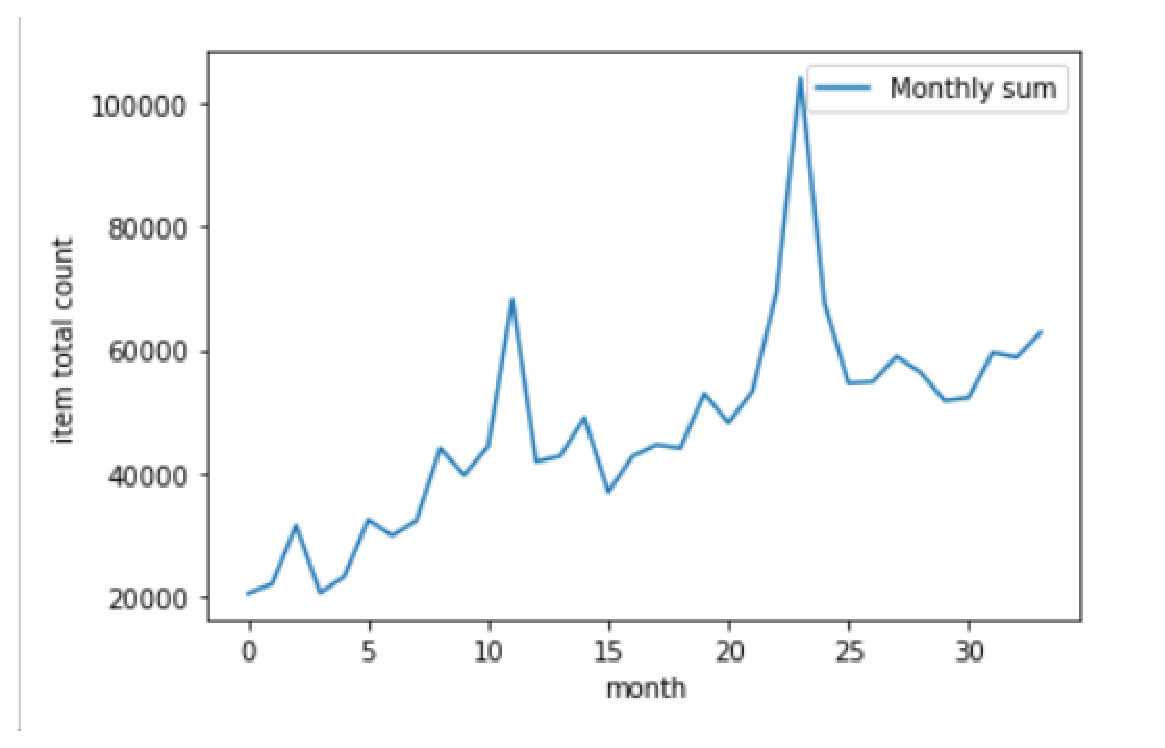
\includegraphics[scale=0.3]{picture/data_20.eps}
        \caption{month_total_count}\label{fig:1}
    \end{figure}
    Explain that the month is related to the sales volume of goods: the sales volume at the end of the year is increasing\par
    Next, take a look at the sales of each store in figure 2\par
    Finally, let's look at the sales of different kinds of goods in figure 3\par
    \textbf{Item and Shop Information:}\par
    large categories, small categories, we separate them, and code them separately to facilitate subsequent feature extraction\par
    \textbf{Shop information:}\par
    the city where the store is located, the type of store, which we separate and encode separately for subsequent feature extraction\par
    \begin{figure}[b]
        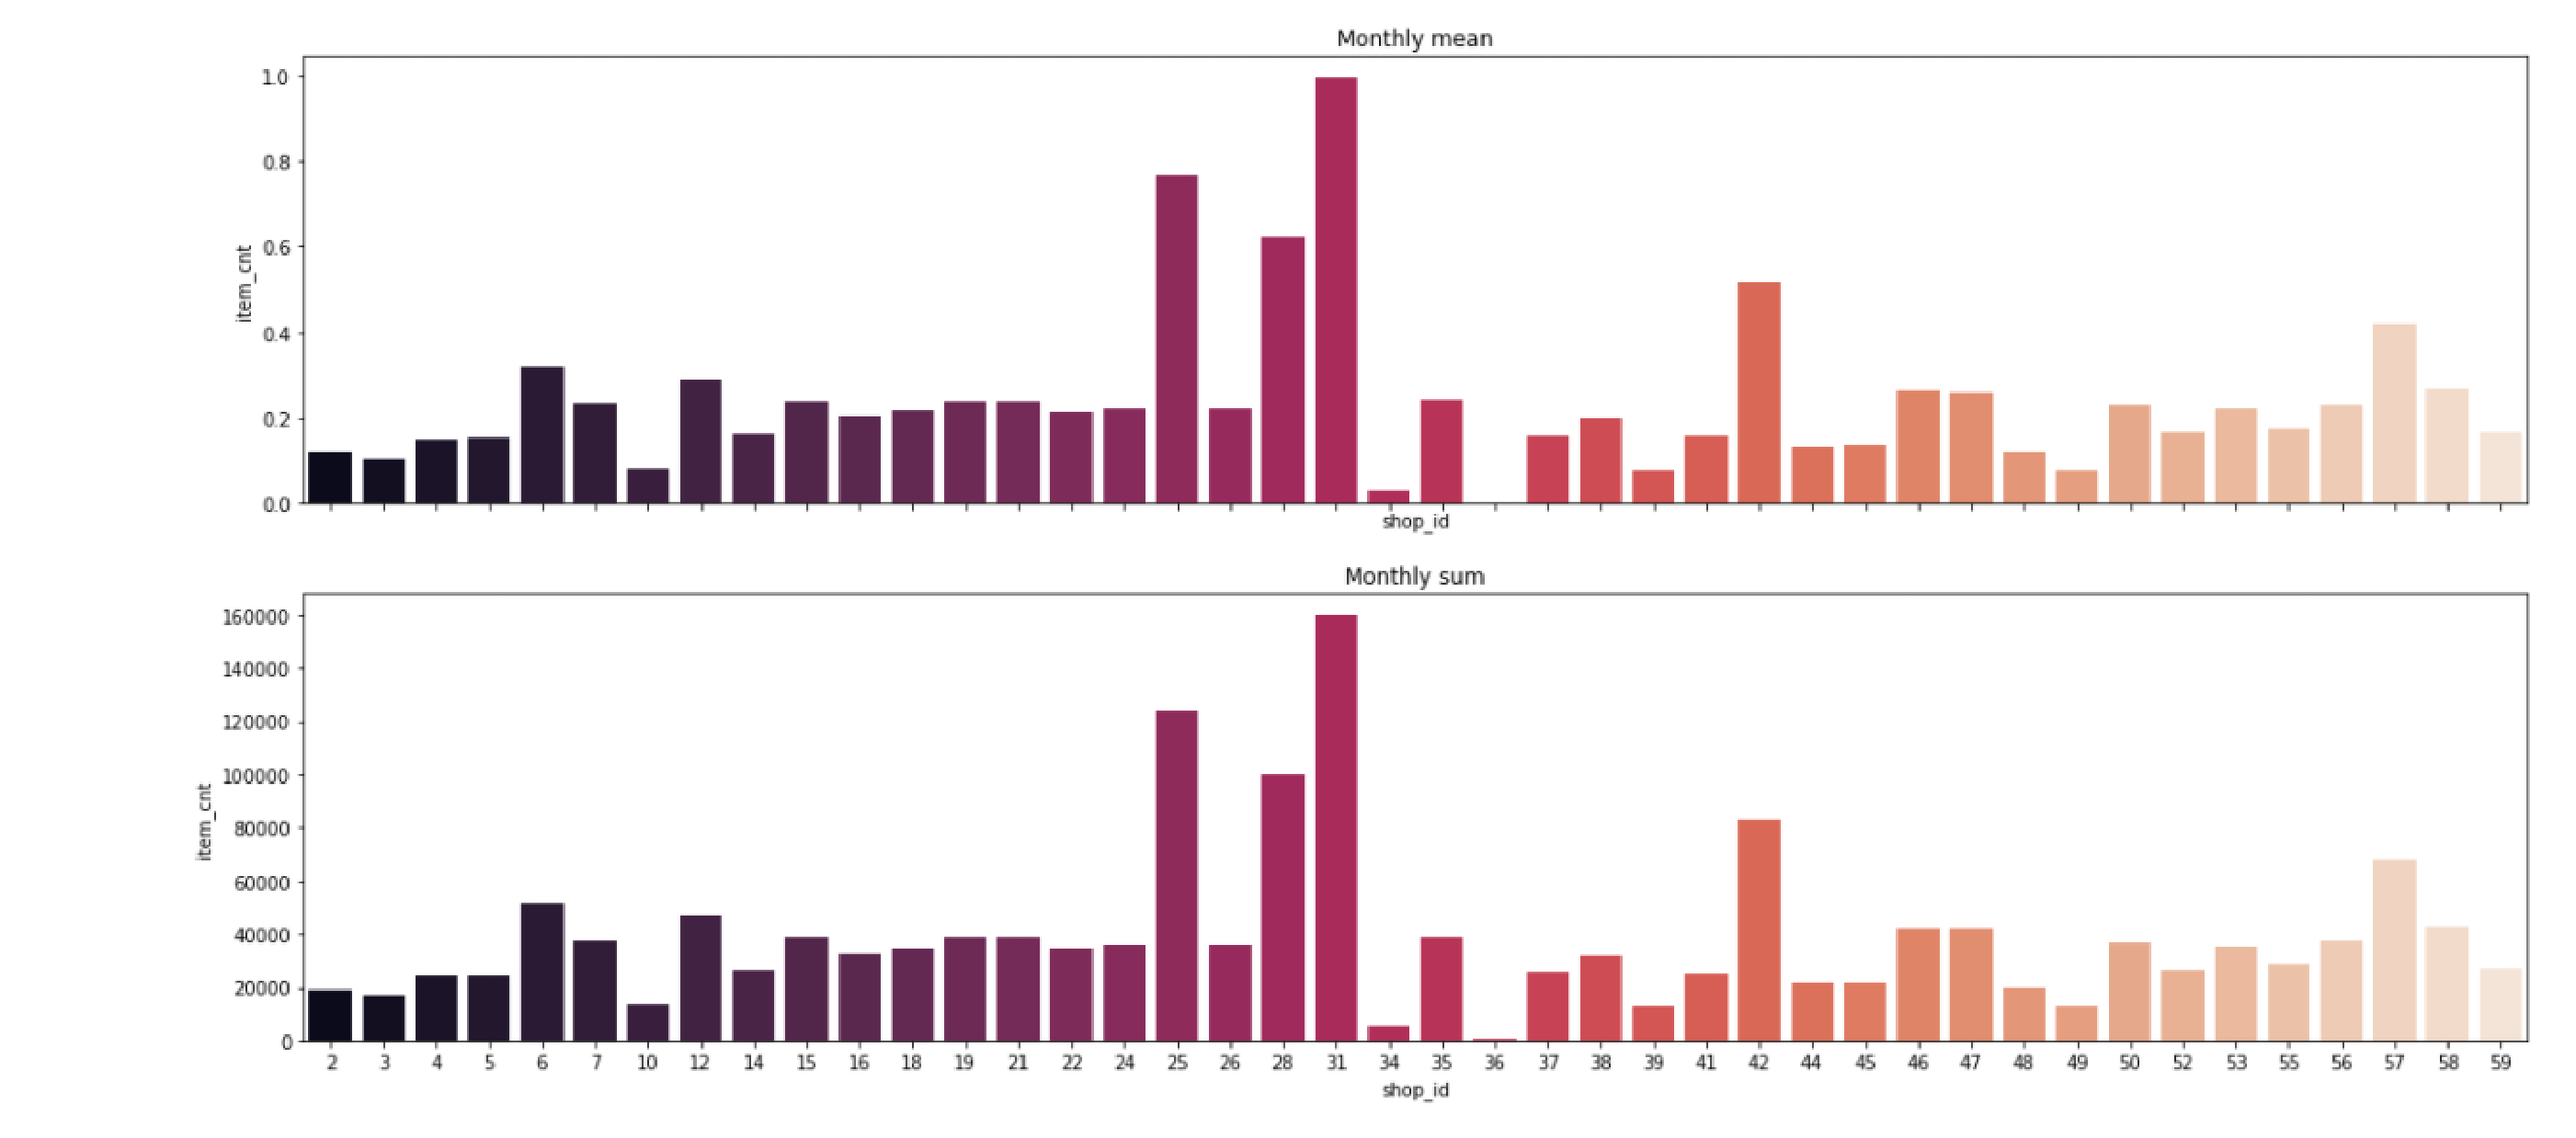
\includegraphics[scale=0.3]{picture/data_30.eps}
        \caption{shop_count}\label{fig:2}
    \end{figure}
    \begin{figure}
        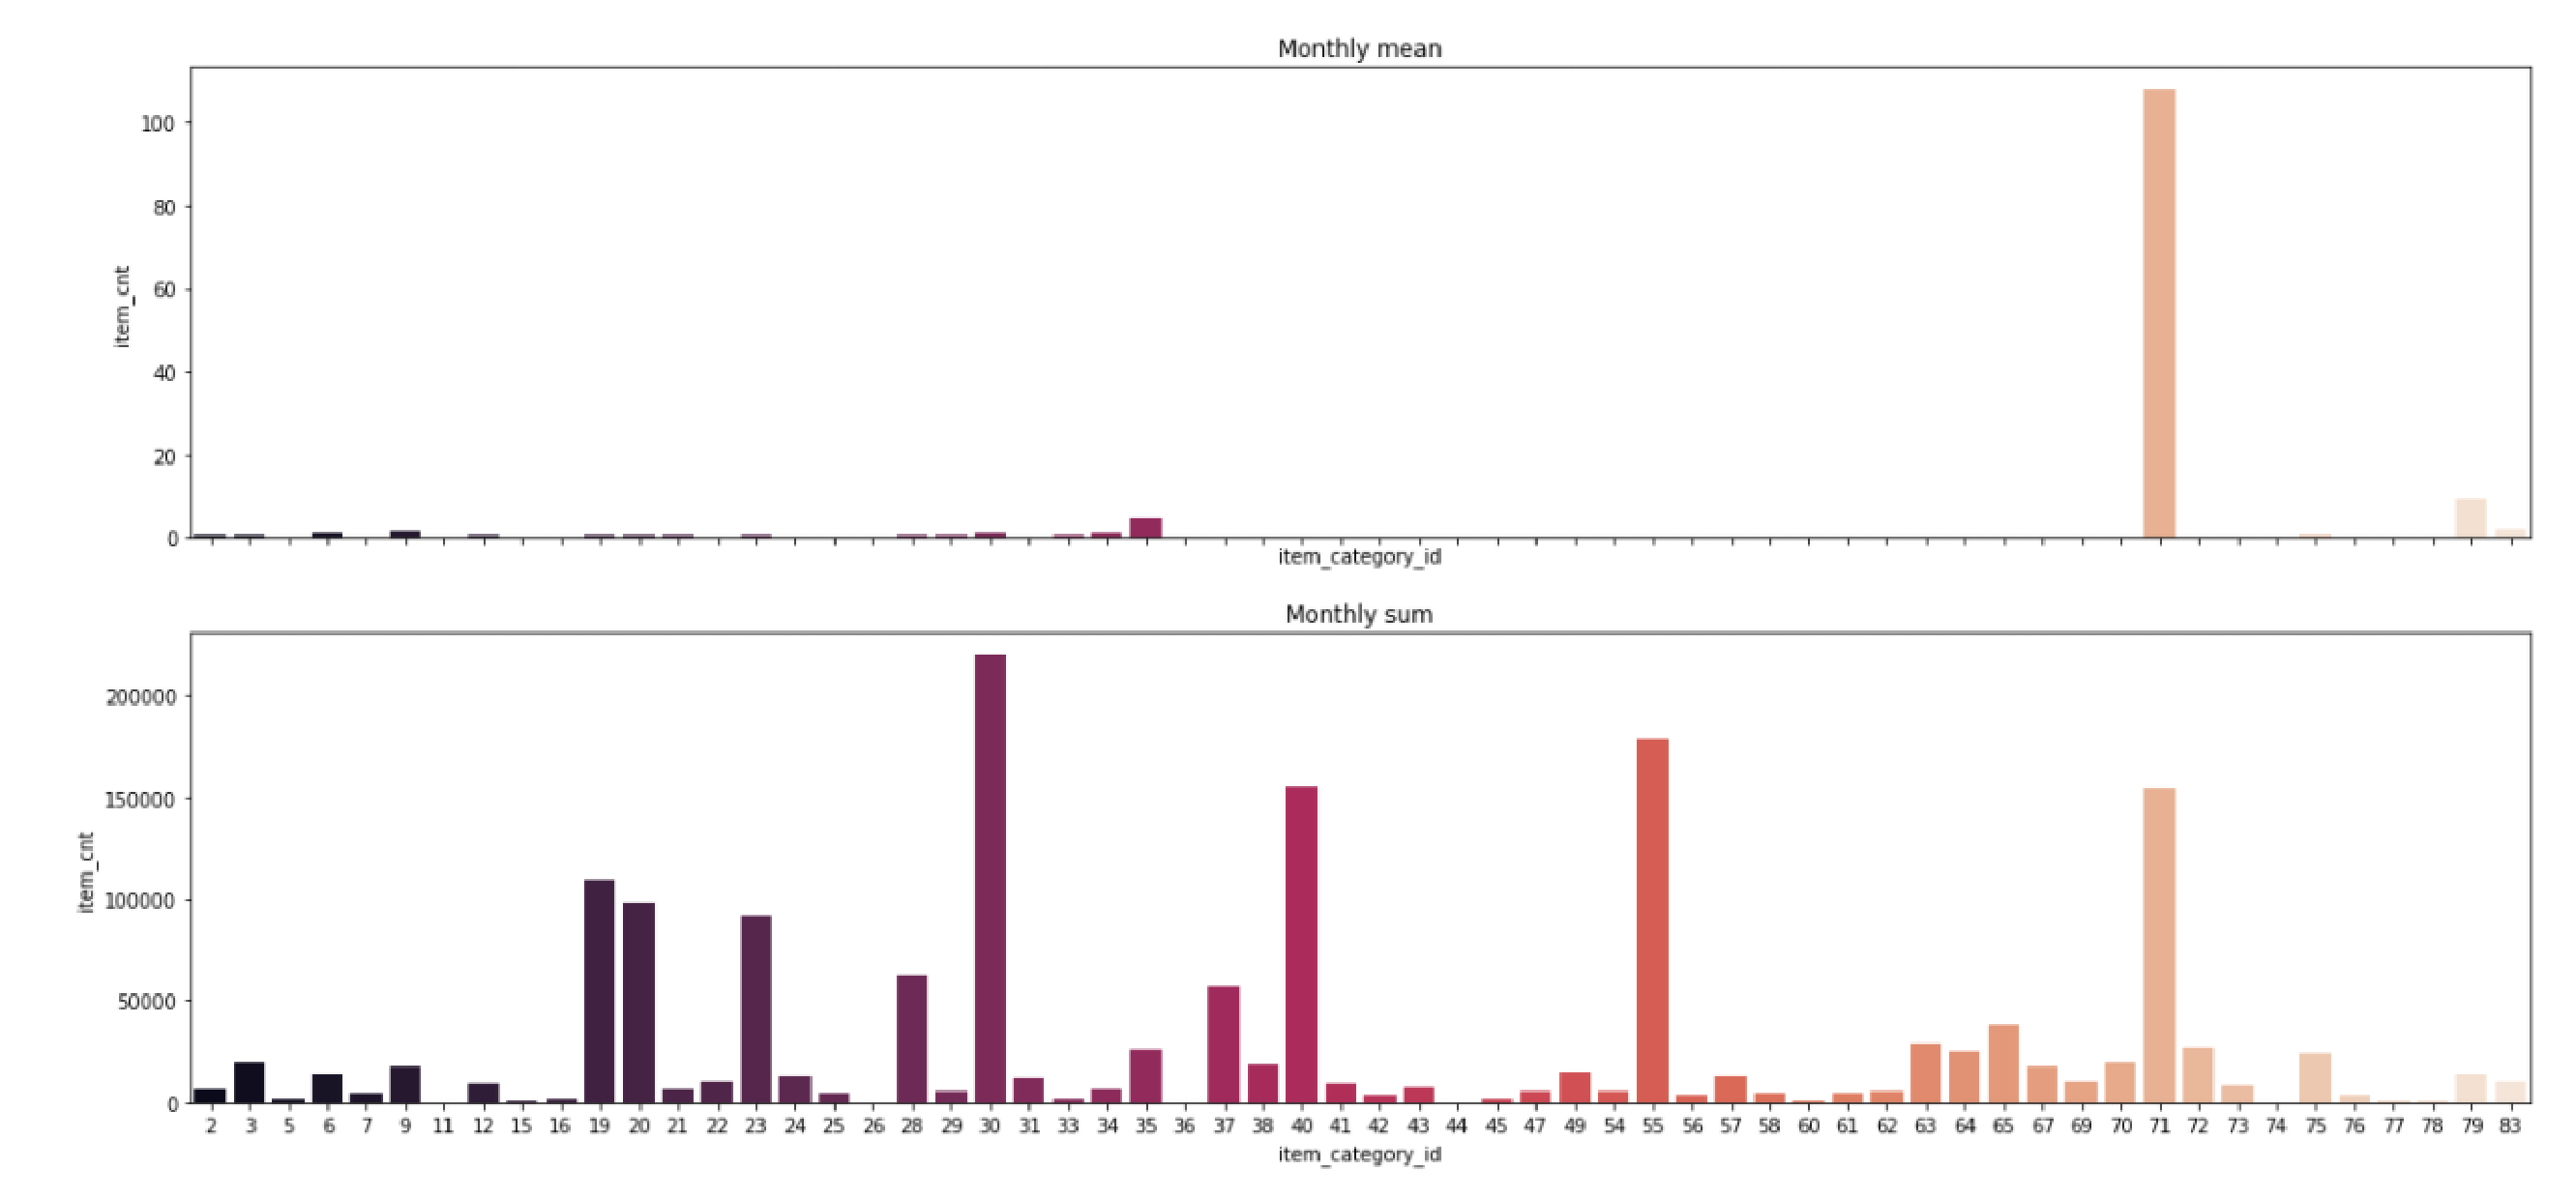
\includegraphics[scale=0.3]{picture/data_31.eps}
        \caption{item_category_count}\label{fig:3}
    \end{figure}
\section{Model}
\subsection{decision tree}\par
In machine learning, decision tree is a prediction model, which represents a mapping relationship between object attributes and object values. Each node in the tree represents an object, and each branch path represents a possible attribute value, while each leaf node corresponds to the value of the object represented by the path from the root node to the leaf node. The decision tree has only a single output, if you want to have complex output, you can establish an independent decision tree to deal with different outputs. Decision tree is a frequently used technology in data mining, which can be used to analyze data, and also can be used for prediction.
\subsection{Candidate model}\par
\begin{itemize}
    \item GBDT
    \item Xgboost
    \item lightgbm
    \item neural network
\end{itemize}
\subsection{Method One}\par
\ 
\newline
The sales of the 34th month are regarded as the sales of the 35th month,Count the sales volume of each item in each store in the 33rd month and merge it with test
The result is \textbf{RMSE=1.16777}
\subsection{Method Two}
\ 
\newline
\textbf{Features:}\par
  \begin{itemize}
    \item shop_id
    \item item_id
    \item item_cnt_month
  \end{itemize}
  The model we choosed is lightgbm,and The result is \textbf{RMSE=}

\subsection{Method Three}\par
\ 
\newline
Adding historical information is good for prediction. We can see the features after adding historical information in Figure 4.
Finally, through experiments, it can be proved that the prediction results are improved.
\textbf{training's rmse: 0.664209,valid_1's rmse: 0.880256}
\begin{figure}
    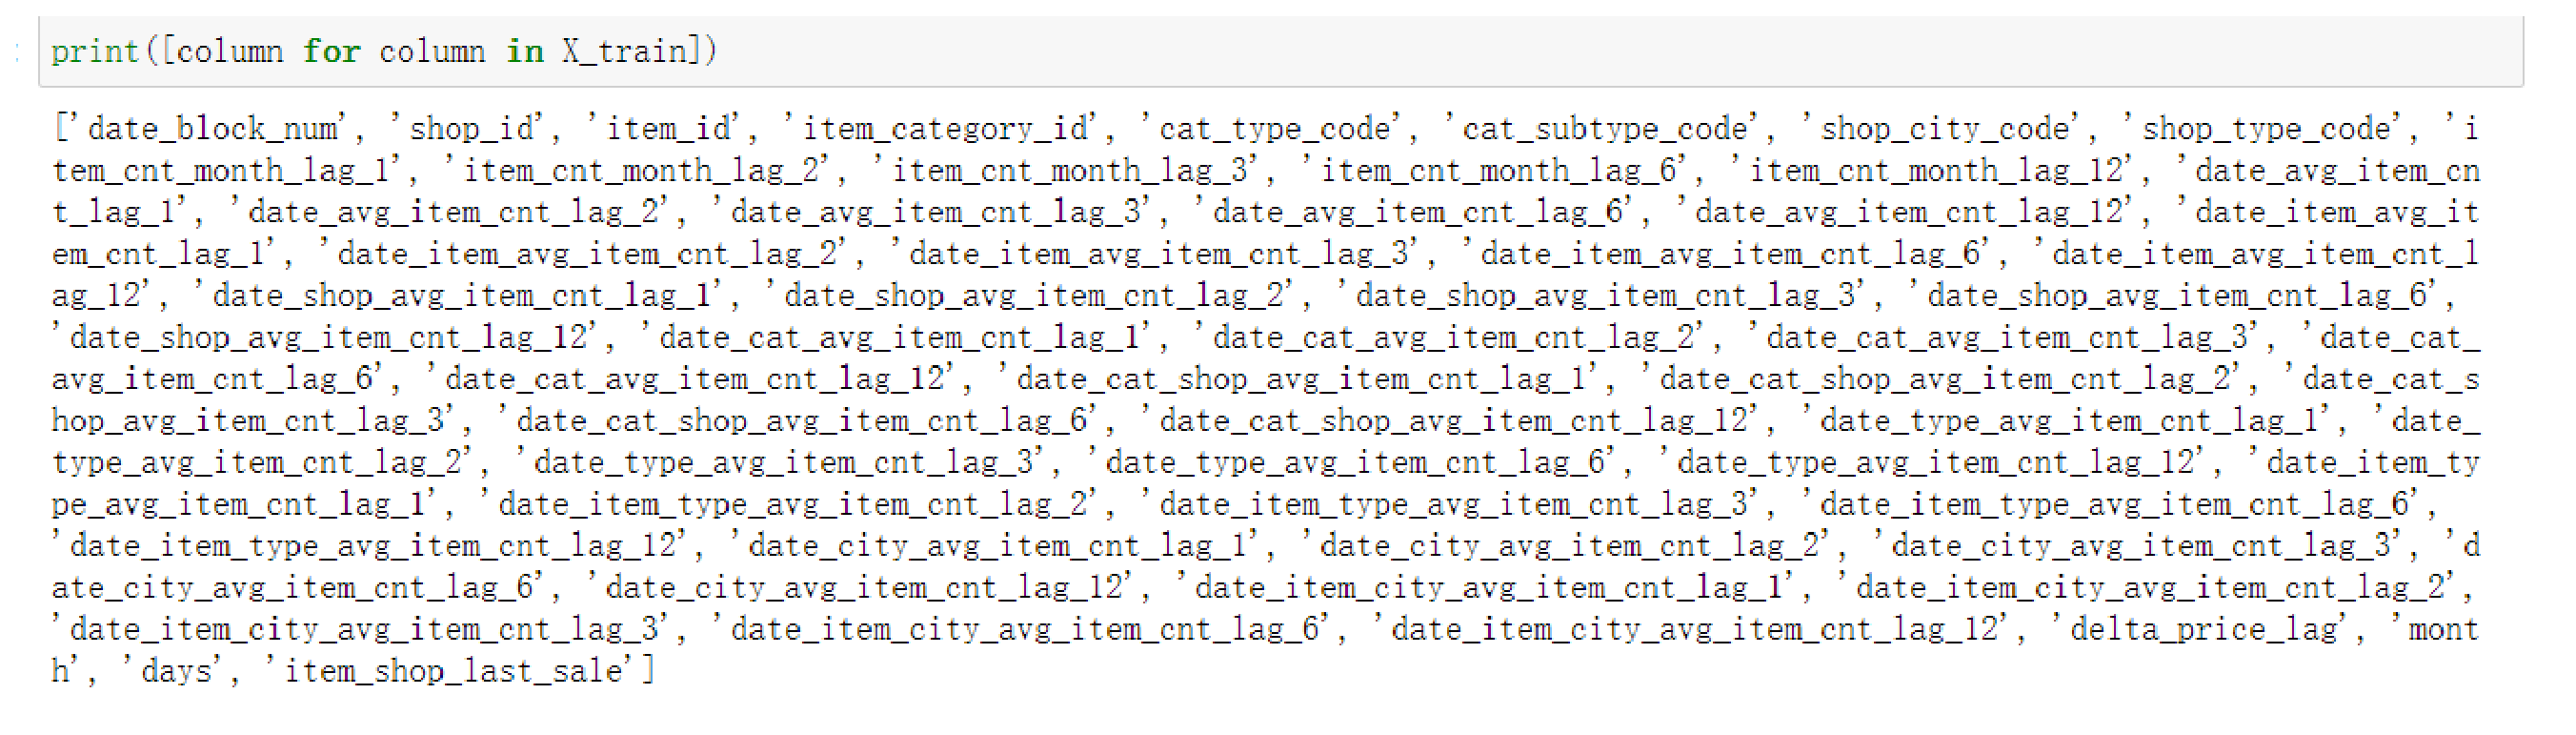
\includegraphics[scale=0.3]{picture/data_16.eps}
    \caption{final features}\label{fig:4}
\end{figure}
\section{Conlusion}
Through data processing and adding delay information, the model achieves good results



\end{document}

